
\section{Probability Distributions}
A probability distribution describes how the values of a random variable are distributed. 

For example, the collection of all possible outcomes of a sequence of coin tossing is known to follow the binomial distribution, whereas the means of sufficiently large samples of a data population are known to resemble the normal distribution (Central limit Theorem). Since the characteristics of these theoretical distributions are well understood, they can be used to make statistical inferences on the entire data population as a whole.

Recall that probability distributions can be categorised as either \textit{\textbf{discrete}} or \textit{\textbf{continuous}}.
We will look at  
\begin{itemize}
\item how to generate random numbers,
\item how to use probability mass and density functions,
\item how to use cumulative distribution functions,
\item how to determine quantiles.
\end{itemize} 

There is a wide variety of probability distributions available, but we shall only look at a few key distribution. 

\begin{itemize}
\item	The Normal Distribution
\item	The Student $t-$Distribution
\item   The Uniform Distribution
\item	The Exponential Distribution
\item	The Binomial Distribution
\item	The Poisson Distribution
\end{itemize}

If you would like to know what distributions are available you can do a search using the command \texttt{\textbf{help.search("distribution")}}. 

%Here we give details about the commands associated with the normal distribution and briefly mention the commands for other distributions. 
%The functions for different distributions are very similar where the differences are noted.


\subsection{Probability Mass Functions} 

For a discrete distribution, the probability mass function (pmf) is the probability that the discrete random variable $X$ has some specified value (k) i.e. $P(X = k)$. Probability mass functions are determined using the \texttt{\textbf{d}} family of functions. For example, for the binomial distribution, the command is \texttt{\textbf{dbinom()}}, for the Poisson distribution \texttt{\textbf{dpois()}}. 

\subsection{Probability Density Functions} 
For a discrete distribution, the probability density function (pdf) is the relative likelihood that the continuous random variable $X$ will have some specified value (k).
Since for continuous distributions the probability at a single point is zero, it is \textbf{not} equivalent to $P(X = k)$.

Rather the density function is the height of a \textbf{\textit{density curve}} (such as the well-known Gaussian bell-curve) at point $k$.

\begin{center}
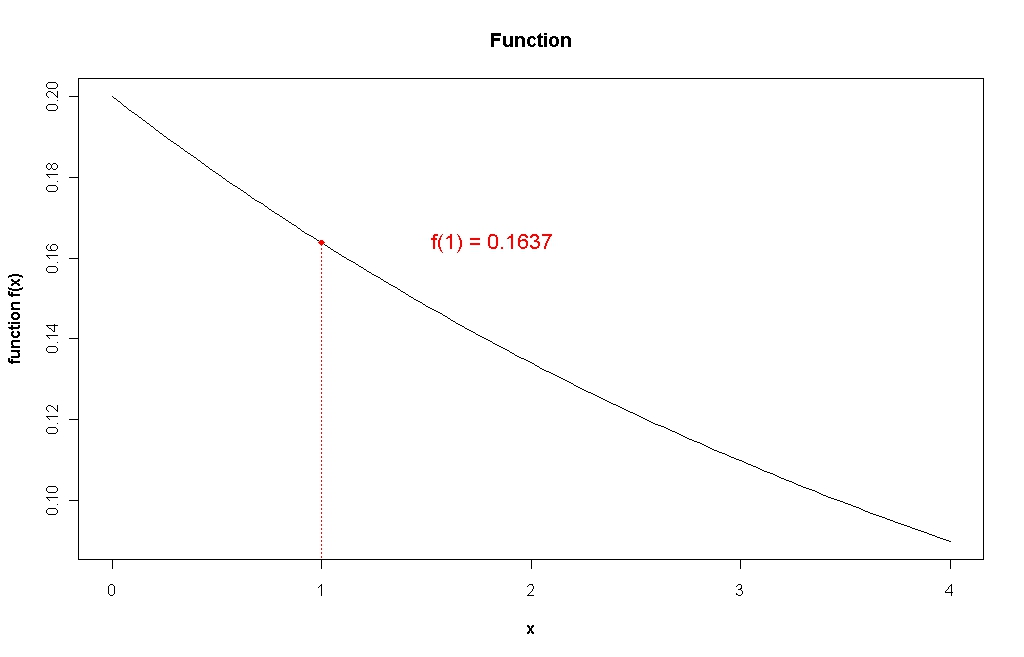
\includegraphics[scale=0.40]{6AFunction}
% \caption{Some function f(x) evaluated at x=1}
\end{center}
 
%\end{document}
 
Probability density functions are determined using the \texttt{\textbf{d}} family of functions. For example, for the normal distribution, the command is \texttt{\textbf{dnorm()}}. 
Necessarily the  \texttt{\textbf{d}} family of functions are more useful for discrete random variables than for continuous variables.

\subsection{Cumulative Distribution Functions}

The cumulative distribution function (cdf) is the probability that the variable takes a value less than or equal to $x$. The cumulative density function is often denoted as $F(x)$.
 
 \[F(x)= P(X \leq x) = \alpha \]

There is little difference in how to treat the cdf for discrete and continuous variables, other than the definition of the complement.
Values for the cumulative distribution functioncan be determined using the \texttt{\textbf{p}} family of functions. 

It is possible to specify the complement probability of the cumulative distribution function (i.e $P(X \geq x)$) directly by additionally specifying the argument \texttt{\textbf{lower=FALSE}}.
 
\subsection{Inverse Cumulative Distribution Functions}

The inverse cumulative distribution function (otherwise known as the quantile function) is a function that yields the quantile $k$ for some specified probability $\alpha$ such that the variable takes a value less than or equal to $k$ with this probability (Recall that $p(X \leq x) = \alpha $).

\[F^{-1}(\alpha) = x  \]

Implementation of the inverse cumulative distribution function requires use of the \texttt{\textbf{q}} family of functions. Quantile functions generally tend to be used with continuous random variables, rather than for discrete random variables.
\newpage
\section{The Normal Distribution}

There are four functions that can be used to generate the values associated with the normal distribution.  
The first function we shall look at is \textbf{\texttt{dnorm}}. Given an appropriate set of argument values (i.e. for mean and standard deviation), this function returns the height of the desnity curve (i.e. plot of the probability density distribution) for those specifications. 

To specify a value for mean, use the argument \textbf{\texttt{mean=}}. Similarly to specify a value for mean, use the argument \textbf{\texttt{sd=}}.

\begin{framed}
\begin{verbatim}
dnorm(3,mean=2,sd=1)
\end{verbatim}
\end{framed}
\begin{verbatim}
> dnorm(3,mean=2,sd=1)
[1] 0.2419707
\end{verbatim}
The default values for mean ($\mu$) and standard deviation ($\sigma$) are 0 and 1 respectively. This is , by definition, the standard normal distribution, commonly called the $Z$ distribution. Therefore, if the values for mean and standard deviation are not specified, 0 and 1 are used by default.
\begin{verbatim}
> dnorm(3)
[1] 0.004431848
> dnorm(0)
[1] 0.3989423
>dnorm(0)*sqrt(2*pi)
[1] 1
> vec = c(0,1,2)
> dnorm(vec)
[1] 0.39894228 0.24197072 0.05399097
\end{verbatim}
The command \texttt{\textbf{dnorm()}} can be used to plot the bell curve. The bell curve depicted below can be constructed using the following \texttt{R} code.
\begin{framed}
\begin{verbatim}
x = seq(-5,5,by=.01)
y = dnorm(x) 
plot(x,y,type="l",lwd=2,col="red")
abline(h=0)
abline(v=0)
\end{verbatim}
\end{framed}
 \begin{center}
 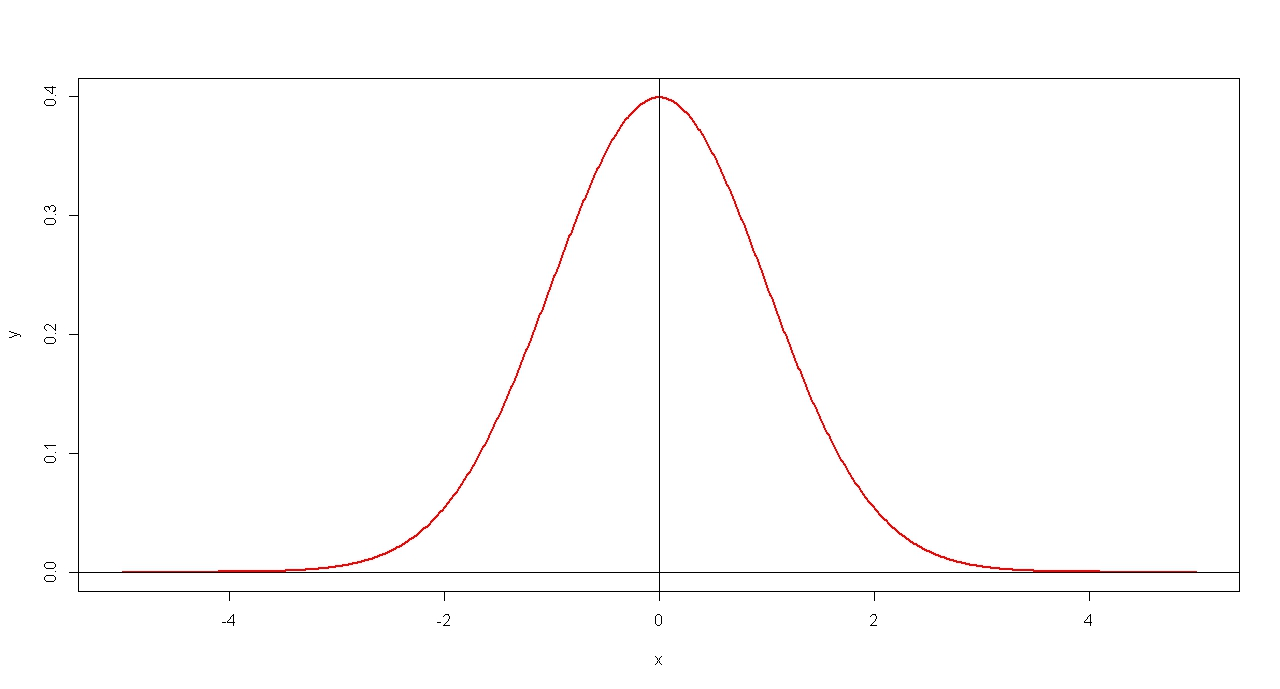
\includegraphics[scale=0.30]{dnormCurve}
% \caption{Some function f(x) evaluated at x=1}
 \end{center}
 

The second function we examine is \texttt{\textbf{pnorm()}}. Given a number or a list this function computes the cumulative distribution function, i.e. probability that a normally distributed random number will be less than that number. This function accepts the same options as \texttt{\textbf{dnorm()}}, i.e. \texttt{\textbf{mean=}} and \texttt{\textbf{sd=}}.


You can get a full list of them and their options using the help command:

\begin{verbatim}
>  pnorm(0)
[1] 0.5
>  pnorm(1)
[1] 0.8413447
>  pnorm(0,mean=2)
[1] 0.02275013
>
>  pnorm(0,mean=2,sd=3)
[1] 0.2524925
>
>  vec = c(0,1,2)         
>  pnorm(vec)
[1] 0.5000000 0.8413447 0.9772499
>
\end{verbatim}
\subsection{Applications of the Normal Distribution}
Suppose the mass of shire horses is assumed to have a normal distribution with mean 1000kg and standard deviation 50kg. 
\begin{enumerate}
\item Calculate the probability that the mass of a shire horse is less than 975kgs.
\item Calculate the probability that the mass of a shire horse is more than 975kgs.
\item Calculate the probability that the mass of a shire horse is between 940kg and 1030kg.         
\item Calculate the probability that the mass of a shire horse exceeds 1030kg.                
\end{enumerate}

Solutions: Let X be the mass of the horses, distributed as
\[ X \sim \mathcal{N}(1000,50^2)\].
\begin{enumerate}
\item $P(X \leq 975)$ : \texttt{\textbf{pnorm(975,mean=1000,sd=50)}}.
\item $P(X \geq 975)$ =  $ 1- P(X \leq 975)$:\texttt{\textbf{1-pnorm(975,mean=1000,sd=50)}}. 
\item $P(940 \leq X \leq 1030)$ = $P(X \leq 1030) -  P(X \leq 940)$  : \texttt{\textbf{pnorm(1030,mean=1000,sd=50)}} - \texttt{\textbf{pnorm(940,mean=1000,sd=50)}}.     
\item $P(X \geq 1030)$       \texttt{\textbf{pnorm(1030,mean=1000,sd=50,lower=FALSE)}}.
\end{enumerate}
\begin{verbatim}
> pnorm(975,mean=1000,sd=50)
[1] 0.3085375
> 1-pnorm(975,mean=1000,sd=50)
[1] 0.6914625
> pnorm(1030,mean=1000,sd=50)-pnorm(940,mean=1000,sd=50)
[1] 0.6106772
>
> pnorm(1030,mean=1000,sd=50)
[1] 0.7257469
> pnorm(1030,mean=1000,sd=50,lower=FALSE)
[1] 0.2742531



\end{verbatim}
The answers are $30.85\%,69.14\%$ and $61.06\%$ respectively.

The next function we look at is \texttt{\textbf{qnorm()}}, which is the inverse of \texttt{\textbf{pnorm()}}. The idea behind \texttt{\textbf{qnorm()}} is that you specify the probability, and it returns the number whose cumulative distribution matches the probability. 
For example, if you have a normally distributed random variable with mean zero and standard deviation one, then if you give the function a probability it returns the associated Z-value:


\begin{verbatim}
> qnorm(0.5)
[1] 0
>#Well Known Z Scores
> qnorm(0.95)
[1] 1.644854
> qnorm(0.975)
[1] 1.959964
> qnorm(0.995)
[1] 2.575829
>
> qnorm(0.5,mean=1)
[1] 1
>  qnorm(0.5,mean=1,sd=2)
[1] 1
>  qnorm(0.5,mean=2,sd=2)
[1] 2
>  qnorm(0.5,mean=2,sd=4)
[1] 2
>  qnorm(0.25,mean=2,sd=2)
[1] 0.6510205
> 
\end{verbatim}

The last function we examine is the  \textbf{\texttt{help(rnorm)}} function which can generate normally distributed random numbers. The argument that must be specified are the number of random numbers required, as well as optional arguments to specify the mean and standard deviation. Randomly generated numbers will be specified to several decimal places, so it is worth recalling functions such as \textbf{\texttt{help(round())}} that can be used to manage precision.
\begin{verbatim}
>  rnorm(4)
[1] -0.79949714 -1.14181543  0.09373155 -0.18318997
>
>  rnorm(4,mean=3)
[1] 3.948279 4.214592 1.488769 1.354725
>
>  rnorm(4,mean=3,sd=3)
[1] 1.259427 1.554388 1.654530 1.076075
> 
>  rnorm(4,mean=3,sd=3)
[1] 2.802254 2.681757 1.528246 6.496170
> 
\end{verbatim}

The help file for thes commands can be obtained by specifying any one of the fuctions as an argument to the \textbf{\texttt{help()}} function: e.g.\textbf{\texttt{help(dnorm)}}.
\newpage
\section{Student t-Distribution}
The Student’s t-distribution is a probability distribution that is used to estimate population parameters when the sample size is small and/or when the population variance is unknown.
The parameters are the \textbf{\textit{degrees of freedom}} (df = n-1 where n is sample size).

As with the normal distribution, there are four functions that can be used to generate the values associated with the $t-$distribution.The commands follow the same kind of naming convention, and the names of the commands are \texttt{\textbf{dt(), pt(), qt()}} and \texttt{\textbf{rt()}}.

One difference between the $t-$distribution and the normal distribution is that, for the $t-$distribution, it is assumed that the values are \textit{\textbf{standardized }}to mean zero and standard deviation one.
Also the number of degrees of freedom must be specified. 

\begin{verbatim}
> pt(-3,df=10)
[1] 0.006671828
>  pt(3,df=10)
[1] 0.9933282
>  1-pt(3,df=10)
[1] 0.006671828
>  pt(3,df=20)
[1] 0.9964621
\end{verbatim}
The density curves for various degrees of freedom (red with df=5, blue with df=15 and green with df=100) are depicted on the following graph.
\begin{framed}
\begin{verbatim}
x = seq(-5,5,by=.01)
y = dt(x,df=100) 
plot(x,y,type="l",lwd=2,col="red")
abline(h=0)
w = dt(x,df=10) 
points(x,w,type="l",lwd=2,col="green",add=TRUE)
z = dt(x,df=5) 
points(x,z,type="l",lwd=2,col="blue",add=TRUE)
\end{verbatim}
\end{framed}
 \begin{center}
 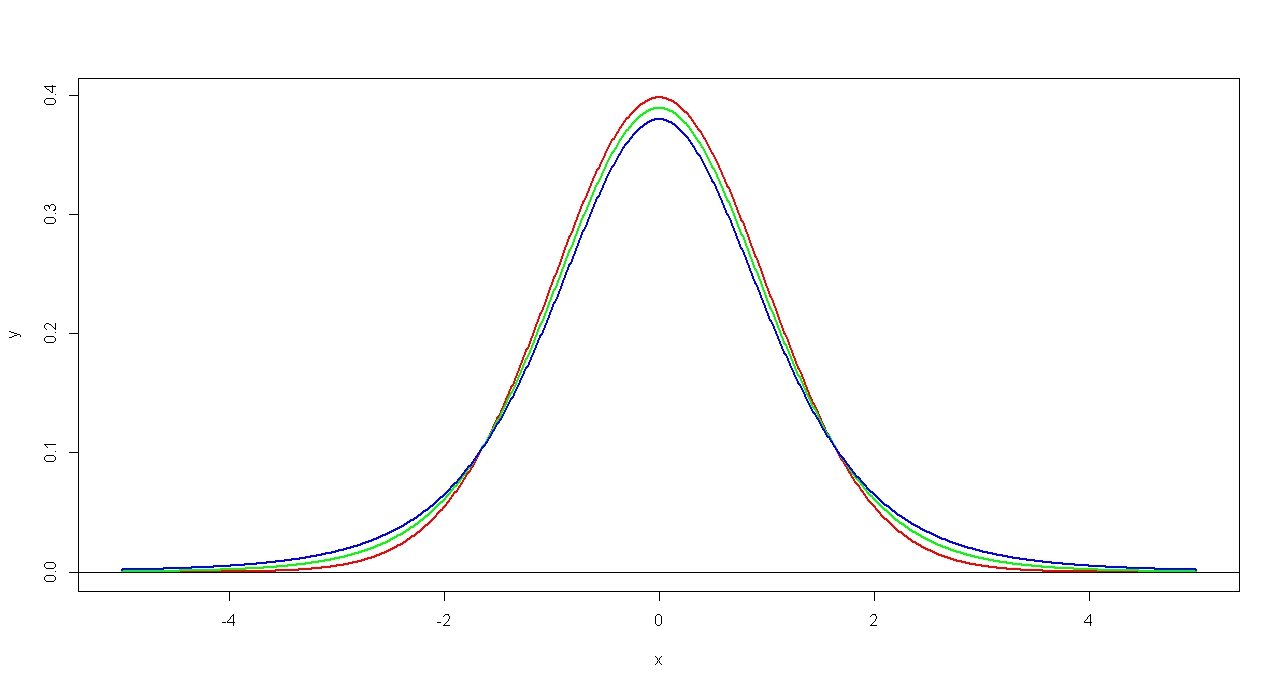
\includegraphics[scale=0.30]{dtCurve}
% \caption{Some function f(x) evaluated at x=1}
 \end{center}
Next we have the inverse cumulative probability distribution function. Recall computing critical values for small sample hypothesis tests. The values computed here are equivalent of the value found in statistical tables.

\begin{verbatim}
> qt(0.05,df=10)
[1] -1.812461
>  qt(0.95,df=10)
[1] 1.812461
>  qt(0.05,df=20)
[1] -1.724718
>  qt(0.95,df=20)
[1] 1.724718
\end{verbatim}
Finally random numbers can be generated according to the $t-$distribution using the \textbf{\texttt{rt()}}.
\begin{verbatim}
> rt(3,df=10)
[1] 0.9440930 2.1734365 0.6785262
> rt(3,df=20)
[1] 0.1043300 -1.4682198  0.0715013
\end{verbatim}







\section{Discrete Probability Distributions}
The discrete distributions we will look at in this course are
\begin{itemize}
\item The binomial distribution
\item The Poisson distribution
\end{itemize}
\subsection{Binomial Distribution}

A binomial experiment (known as a Bernoulli trial) is a statistical experiment that has the following properties: 

\begin{itemize}
\item	The experiment consists of $n$ repeated trials.
\item	Each trial can result in just two possible outcomes. We call one of these outcomes a success and the other, a failure.
\item	The probability of success, conventionally denoted mathematically as $p$, is the same on every trial.
\item	The trials are independent; that is, the outcome on one trial does not affect the outcome on other trials.
\item	There are $n$ independent trials.
\end{itemize}
 

As with other functions, there are four functions that can be used to generate the values associated with the binomial distribution; \textbf{\texttt{dbinom()}},\textbf{\texttt{pbinom()}}, \textbf{\texttt{qbinom()}} and \textbf{\texttt{rbinom()}}.
The arguments to these commands are \texttt{\textbf{size=}} and \texttt{\textbf{prob=}}.

Suppose that there are ten independent trials, and that the probability of success on each trial is 0.6, the probability of 5 successes over ten trials can be computed using the following code.
\begin{framed}
\begin{verbatim}
dbinom(5,size=10,prob=0.60)
\end{verbatim}
\end{framed}
The probability that the numbers not excessing 5 successes is computed using the \textbf{\texttt{pbinom()}} function.
\begin{framed}
\begin{verbatim}
pbinom(5,size=10,prob=0.60)
\end{verbatim}
\end{framed}

\begin{verbatim}
> dbinom(5,size=10,prob=0.60)
[1] 0.2006581
> pbinom(5,size=10,prob=0.60)
[1] 0.3668967
\end{verbatim}

 \begin{center}
 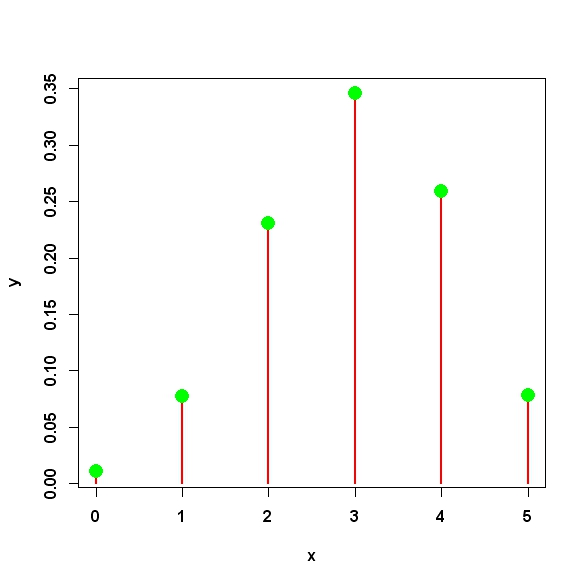
\includegraphics[scale=0.50]{dbinomPlot}
% \caption{Some function f(x) evaluated at x=1}
 \end{center}
 
This plot was implemented with the following \texttt{R} code.
\begin{framed}
\begin{verbatim}
x = seq(0,5,by=1)
y = dbinom(x,5,0.6)
plot(x,y,type="h",col="red",lwd=2,font.lab=2,font.axis=2)
points(x,y,type="p",col="green",cex=2,pch=16)
\end{verbatim}
\end{framed}
The heights of each line are as follows:
\begin{verbatim}
> dbinom(0:5,size=5,prob=0.60)
[1] 0.01024 0.07680 0.23040 0.34560 0.25920 0.07776
\end{verbatim}

\subsubsection{Exercise}
Suppose there are twelve multiple choice questions in an English class quiz. Each question has five possible answers, and only one of them is correct. Find the probability of having four or less correct answers if a student attempts to answer every question at random. 

\textbf{Solution:} Since only one out of five possible answers is correct, the probability of answering a question correctly by random is 1/5=0.2. To find the probability of having four or less correct answers by random attempt, we apply the function pbinom with x = 4, size = 12, prob = 0.2. 

\begin{verbatim}
> pbinom(4, size=12,prob=0.2) 
[1] 0.92744 
\end{verbatim}

The probability of four or less questions answered correctly by random in a twelve question multiple choice quiz is 92.7\%. 
 
\subsubsection{Generating Random Values}

Suppose we wish to simulate the number of defective components in a sequence of twenty batches of 100 items, where the probability of defect is 0.02. We would implement this simulation as follows:

\begin{framed}
\begin{verbatim}
rbinom(20,size=100,prob=0.02)
\end{verbatim}
\end{framed}

\begin{verbatim}
> rbinom(20,size=100,prob=0.02)
 [1] 0 3 1 1 3 2 0 2 2 0 5 0 1 1 3 1 2 4 0 3
\end{verbatim}
\subsubsection{Quantiles}
The inverse cumulative distribution function can be implemented using the \texttt{\textbf{qbinom()}} function.
However the output is generally not as useful as the \texttt{\textbf{pbinom()}} function.
\begin{verbatim}
> qbinom(0.95,100,0.02)
[1] 5
> qbinom(0.90,100,0.02)
[1] 4
> qbinom(0.80,100,0.02)
[1] 3
> qbinom(0.85,100,0.02)
[1] 3
\end{verbatim}

%---------------------------------------- %
\newpage
\subsection{The Poisson Distribution}

A Poisson distribution is the probability distribution that results from a Poisson experiment. A Poisson experiment, ,with $X$ as the number of successes, is a statistical experiment that has the following properties: 

%\subsubsection{Attributes of a Poisson Experiment}

\begin{itemize}
\item The experiment results in outcomes that can be classified as successes or failures.
\item The average number of successes ($\lambda$ or lambda) that occurs in a specified region is known.
\item The probability that a success will occur is proportional to the size of the region.
\item The probability that a success will occur in an extremely small region is virtually zero. 
\end{itemize}

Note that the specified region could take many forms. For instance, it could be a length, an area, a volume, a period of time, etc. The Poisson distribution will feature significantly in the \textbf{\textit{Stochastic Processes}} module that many of you will study in the future.

There are four functions that can be used to generate the values associated with the Poisson distribution. 
The commands follow the same kind of naming convention, and the names of the commands are \texttt{\textbf{dpois()}}, \texttt{\textbf{ppois()}}, \texttt{\textbf{qpois()}}, and \texttt{\textbf{rpois()}}.

These commands work just like the commands for the other distribution. The Poisson distribution requires the lambda. parameters. A few examples are given below to show how to use the different commands. First we have the density function, \texttt{\textbf{dpois()}}.

\subsubsection{Example}
Suppose that the expected number of occurences per unit space is 5, compute the probability of exactly 4 and exactly 5 occurences, i.e. $P(X = 4)$ and $P(X = 5)$ respectively.

\begin{framed}
\begin{verbatim}
dpois(4,lambda=5)
dpois(5,lambda=5)
\end{verbatim}
\end{framed}
The probability of both 4 and 5 successes is 17.5\%.
\begin{verbatim}
> dpois(4,lambda=5)
[1] 0.1754674
> dpois(5,lambda=5)
[1] 0.1754674
\end{verbatim}

 \begin{center}
 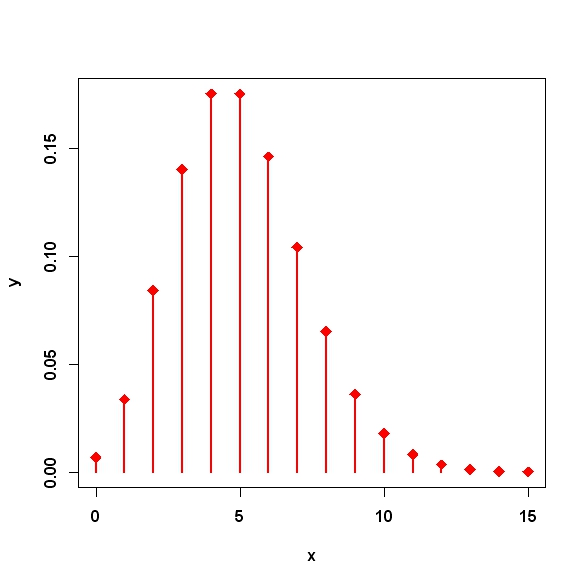
\includegraphics[scale=0.50]{dpoisPlot}
% \caption{Some function f(x) evaluated at x=1}
 \end{center}
 
This plot was implemented with the following \texttt{R} code.
The upper limit of 15 was arbitrarily chosen. There is no upper bound in the sample space of potential successes.
\begin{framed}
\begin{verbatim}
x = seq(0,15,by=1)
y = dpois(x,lambda=5)
plot(x,y,type="h",col="red",lwd=2,font.lab=2,font.axis=2)
points(x,y,type="p",col="red",cex=1.60,pch=18)
\end{verbatim}
\end{framed}
Compute the probability that the number of successes is less than or equal to 15, i.e. $P(X \leq 15)$. To compute this, we would use the \textbf{\texttt{ppois()}} command. The answer is 99.99\%.

\begin{framed}
\begin{verbatim}
ppois(3,lambda=5)
\end{verbatim}
\end{framed}
\begin{verbatim}
> ppois(15,lambda=5)
[1] 0.999931
\end{verbatim}

As mentioned previously, the Poisson distribution is particularly useful in simulating stochastic processes, by generating suitable random values.
Suppose the expected number of occurrences is 5 per month. To simulate the number of occurences for two year (i.e. 24 months), we use the \texttt{\textbf{rpois()}} function.

\begin{verbatim}
> rpois(24,lambda=5)
 [1] 4 6 5 6 5 4 7 7 1 2 3 6 7 1 2 6 2 2 7 9 1 4 5 1
\end{verbatim}

\subsection{Exercise}

If there are twelve cars crossing a bridge per minute on average, find the probability of having seventeen or more cars crossing the bridge in a particular minute (i.e. $P(X\geq 17)$). 

The probability of having sixteen or less cars crossing the bridge in a particular minute is given by the  \texttt{\textbf{ppois()}} function. 
\begin{verbatim}
> ppois(16, lambda=12)   
[1] 0.89871 
\end{verbatim}

Hence the probability of having seventeen or more cars crossing the bridge in a minute is in the upper tail of the probability density function. 
\begin{verbatim}
> ppois(16, lambda=12, lower=FALSE)   # upper tail 
[1] 0.10129 
\end{verbatim}

If there are twelve cars crossing a bridge per minute on average, the probability of having seventeen or more cars crossing the bridge in a particular minute is 10.1\%. 







%----------------------------------------------------------------- %
\section{Summary of Distributions}
\begin{center}
\begin{tabular}{|c|c|c|}
\hline
Distribution &	R name & Arguments\\ \hline
beta &	beta &	shape1, shape 2, ncp\\
binomial &	binom	& size, prob\\
Cauchy	& cauchy	& location, scale\\
chi-squared &	chisq &	df, ncp\\
exponential	& exp &	rate\\
F	& f	& df1,df2,ncp\\
normal &	norm &	mean, sd\\
Poisson&	pois & 	lambda\\
Student's t	& t&	df, ncp\\
uniform	& unif &	min, max\\
Weibull	& weibull & shape, scale\\
Wilcoxon &	wilcox &	m, n\\ 
\hline 
\end{tabular}
\end{center}
 
 \end{document}
%----------------------------------------------------------------- %





